% Figure source. `npm run notes -- build stat497` compiles it to the PDF the
% notes include and to sample-paths.svg for the web page. Values are the ones
% read off the handwritten chart; Monday to Wednesday match the table. The
% chart labels its highlighted line omega_3, but the values it plots are
% scenario omega_2's, so it is labelled omega_2 here.
\documentclass[tikz,border=4pt]{standalone}
\usepackage{libertinus}
\usepackage{libertinust1math}
\usepackage{pgfplots}
\pgfplotsset{compat=1.18}
\definecolor{accent}{HTML}{1D4E89}
\definecolor{caution}{HTML}{9B2C2C}
\definecolor{quiet}{HTML}{6B7280}
\definecolor{hair}{HTML}{D5D9DF}

\begin{document}
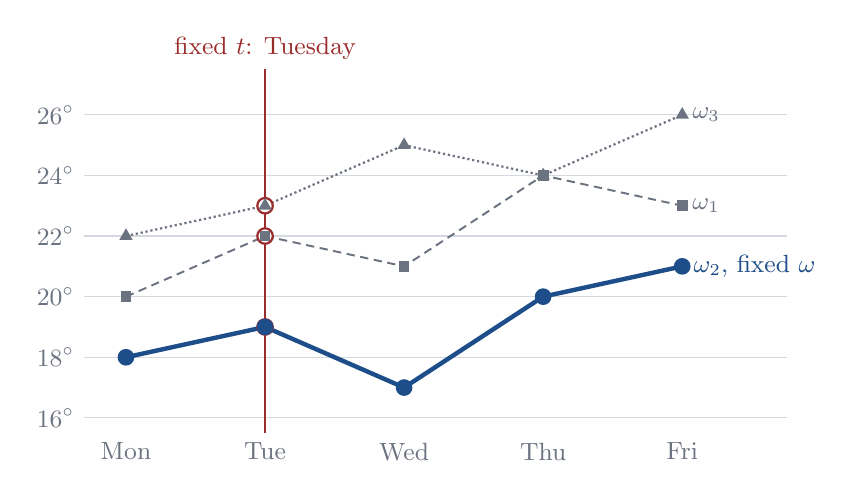
\begin{tikzpicture}
  \begin{axis}[
      width=10.5cm, height=6.2cm,
      xmin=0.7, xmax=5.75, ymin=15.5, ymax=27.5,
      xtick={1,...,5}, xticklabels={Mon,Tue,Wed,Thu,Fri},
      ytick={16,18,...,26}, yticklabel={$\pgfmathprintnumber{\tick}^\circ$},
      axis line style={draw=none}, tick style={draw=none},
      ymajorgrids, grid style={hair, line width=.4pt},
      tick label style={font=\small, text=quiet},
      clip=false,
    ]
    % Fixing the time: one vertical slice through every scenario.
    \draw[caution, line width=.8pt] (axis cs:2,15.5) -- (axis cs:2,27.5)
      node[above, font=\small] {fixed $t$: Tuesday};

    \addplot[quiet, densely dashed, line width=.7pt, mark=square*, mark size=1.6pt,
      mark options={solid}] coordinates {(1,20) (2,22) (3,21) (4,24) (5,23)}
      node[right, font=\small, text=quiet] {$\omega_1$};
    \addplot[quiet, densely dotted, line width=.8pt, mark=triangle*, mark size=2pt,
      mark options={solid}] coordinates {(1,22) (2,23) (3,25) (4,24) (5,26)}
      node[right, font=\small, text=quiet] {$\omega_3$};
    % Fixing the outcome: one whole path through time.
    \addplot[accent, line width=1.6pt, mark=*, mark size=2.2pt]
      coordinates {(1,18) (2,19) (3,17) (4,20) (5,21)}
      node[right, font=\small, text=accent] {$\omega_2$, fixed $\omega$};

    % The random variable at Tuesday: one value per scenario.
    \pgfplotsinvokeforeach{19,22,23}{
      \draw[caution, line width=.8pt, fill=white] (axis cs:2,#1) circle (2.8pt);
    }
  \end{axis}
\end{tikzpicture}
\end{document}
